\documentclass[10pt,a4paper]{article}
\usepackage[a4paper,margin=2.3cm]{geometry}
\usepackage[T1]{fontenc}
\usepackage{newpxtext,newpxmath}
\usepackage{microtype}
\usepackage{CJKutf8}
\newcommand{\jp}[1]{\begin{CJK}{UTF8}{min}#1\end{CJK}}
\usepackage{graphicx}
\usepackage{booktabs,tabularx}
\usepackage{xcolor}
\usepackage{caption}
\usepackage{enumitem}
\usepackage{fancyhdr}
\usepackage[section]{placeins}
\usepackage[colorlinks=true,linkcolor=blue!50!black,citecolor=blue!50!black,urlcolor=blue!50!black,
  pdftitle={What does the Super Mario 64 signpost say?},pdfauthor={mochi64},
  pdfsubject={Forward-model reconstruction of the SM64 wooden signpost texture}]{hyperref}
\usepackage[nameinlink,capitalise]{cleveref}
\captionsetup{font=small,labelfont=bf,margin=0.5em}
\setlist{nosep,leftmargin=1.4em}
\pagestyle{fancy}\fancyhf{}\renewcommand{\headrulewidth}{0.3pt}
\fancyhead[L]{\small What does the Super Mario 64 signpost say?}\fancyhead[R]{\small\thepage}
\graphicspath{{figures/}}
\newcommand{\q}[1]{``#1''}

\title{\vspace{-1.2cm}\textbf{What does the Super Mario 64 signpost say?}\\[0.3em]
\large Reconstructing the tiny text on the wooden signpost texture}
\author{mochi64}
\date{16 October 2026}

\begin{document}
\maketitle
\thispagestyle{empty}

\begin{abstract}
\noindent Every wooden signpost in \emph{Super Mario 64} (1996) carries the same small picture on its front: a
$32{\times}32$ texture with three lines of writing. The letters are only about three pixels tall, so nobody can read
them. We did not try to read them. Instead we rebuilt how such a picture is made (type a text in a font, shrink it,
lay it on painted wood) and searched for the text whose rebuilt picture matches the stored pixels best. We scored
over three billion grammatical candidate signs on a GPU, fitted 2{,}897 period fonts, and finally read the result the
way the Japanese developers would have written it. Our reading is
\begin{center}\Large\textit{I'm here. See}\\\textit{me as you go.}\\\textit{Hold on!}\end{center}
In Japanese this is a typical friendly sign: \jp{ここにいるよ。通りがかりに見ていってね。がんばってね！} The first line is
well supported by the pixels. The second and third lines are only partly fixed by the pixels: we chose the
words that make sense as a whole sentence and as a translation from Japanese. We are open about where the
pixels prefer something else.
\end{abstract}

\begin{figure}[h]\centering
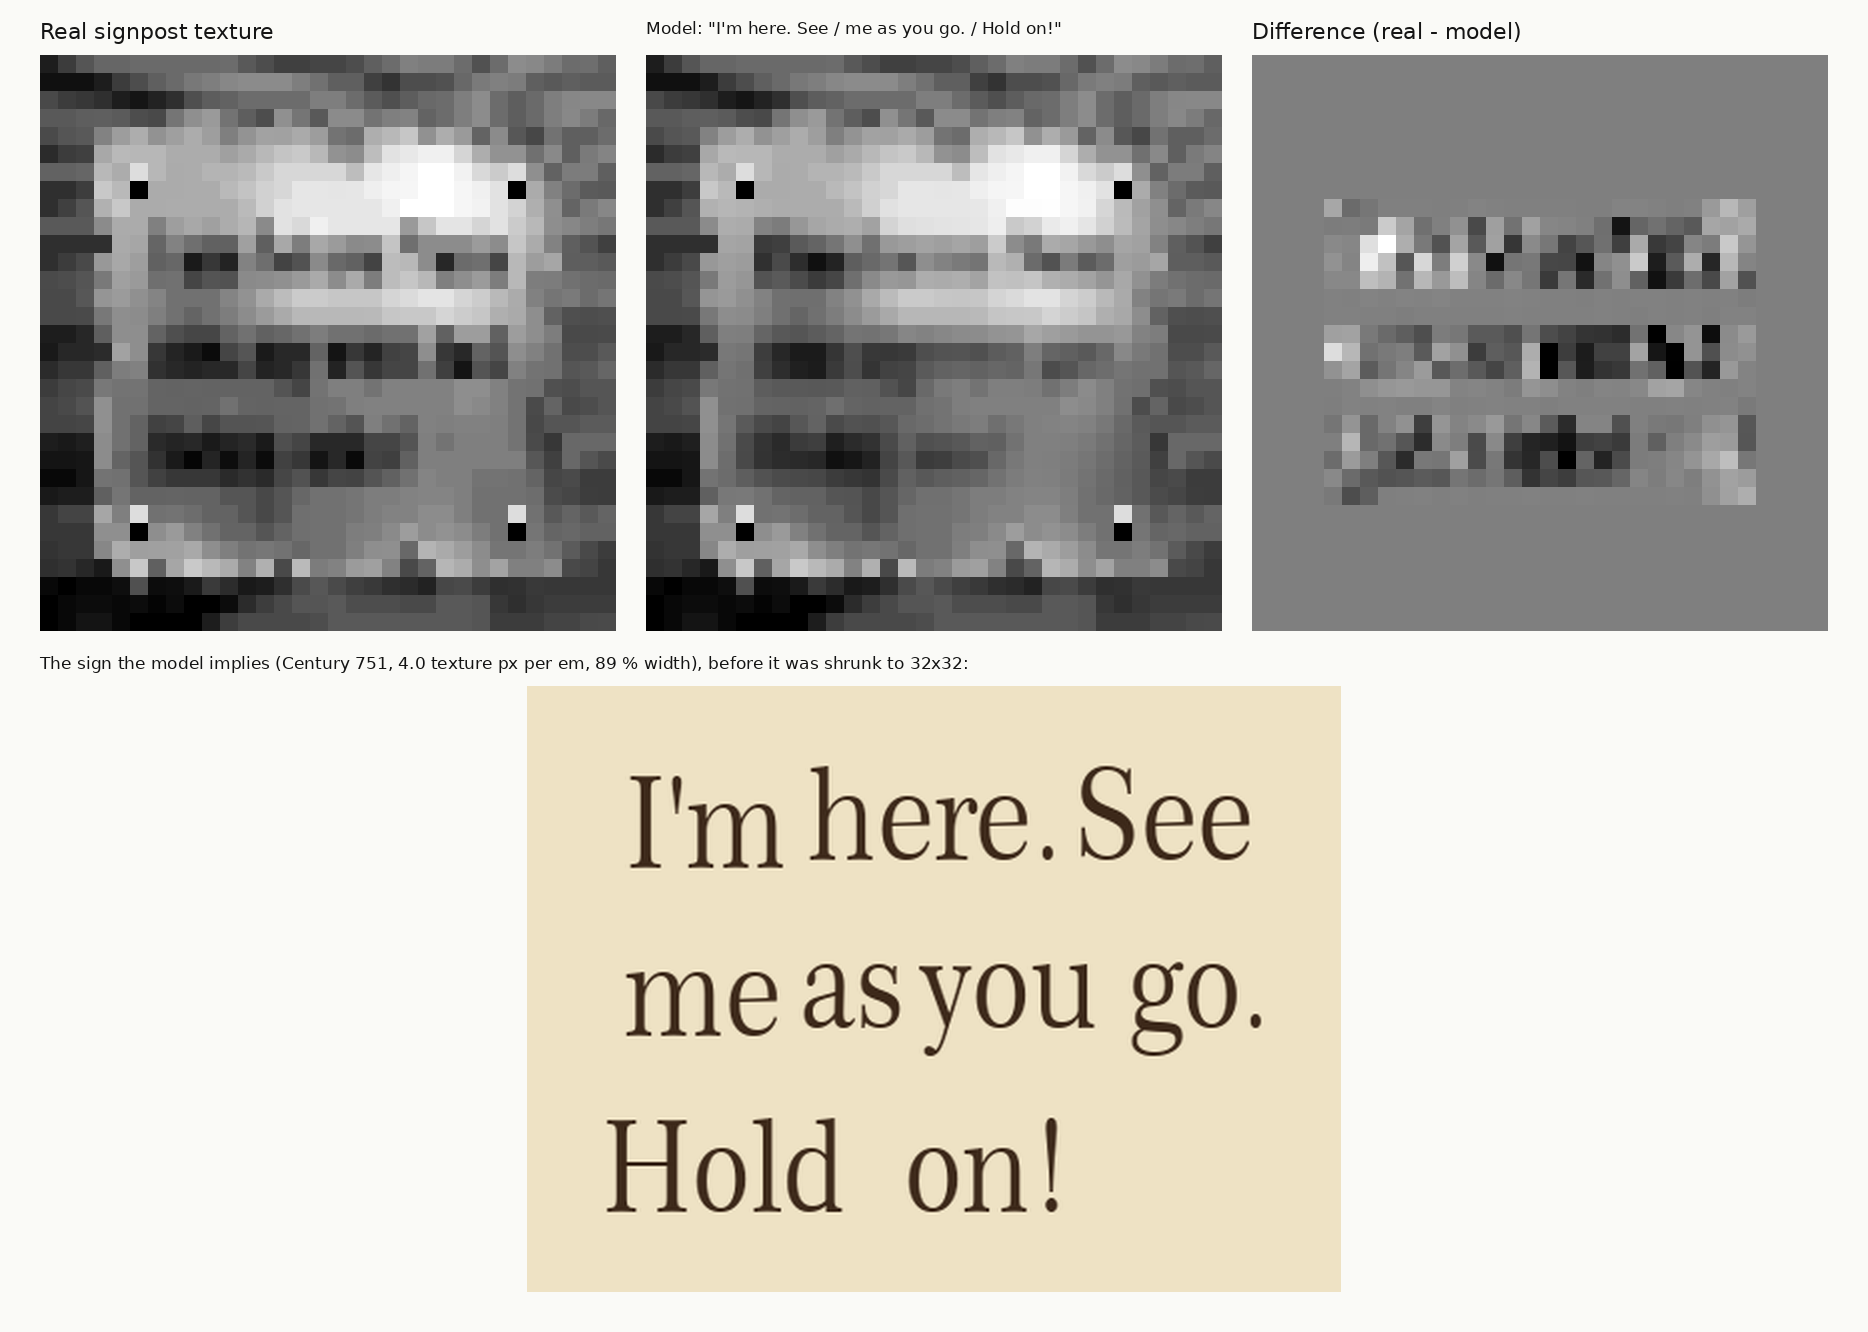
\includegraphics[width=\linewidth]{sign_final.png}
\caption{\textbf{The result in one picture.} Left: the real signpost texture from the game. Middle: our model of how it
was made, with the text \q{I'm here. See / me as you go. / Hold on!}. Right: the difference between the two inside the
three text lines (grey = no difference). Bottom: the sign the model implies before it was shrunk to $32{\times}32$,
set in the font that fits best (Century~751).}
\label{fig:final}
\end{figure}
\clearpage

\section{The sign}
\label{sec:sign}
Signposts are everywhere in \emph{Super Mario 64}: in Bob-omb Battlefield, in the castle grounds, in the snow
levels, in the caves. Mario stands in front of one, presses B, and the sign \q{speaks}. All of them use the same front
picture (the game file is called \texttt{wooden\_signpost\_front}): a small, light board on wood with three short
lines of dark writing (\cref{fig:texture}, left). The writing is decoration. What the game says when you read a sign is
stored separately as dialog text; for the writing on the board itself we know of no reading.

The picture is only $32{\times}32$ pixels. The letters are about three pixels tall, so each letter is a handful of grey
pixels. Looking harder, upscaling or sharpening does not help: at this size any reader sees whatever they expect.

\begin{figure}[h]\centering
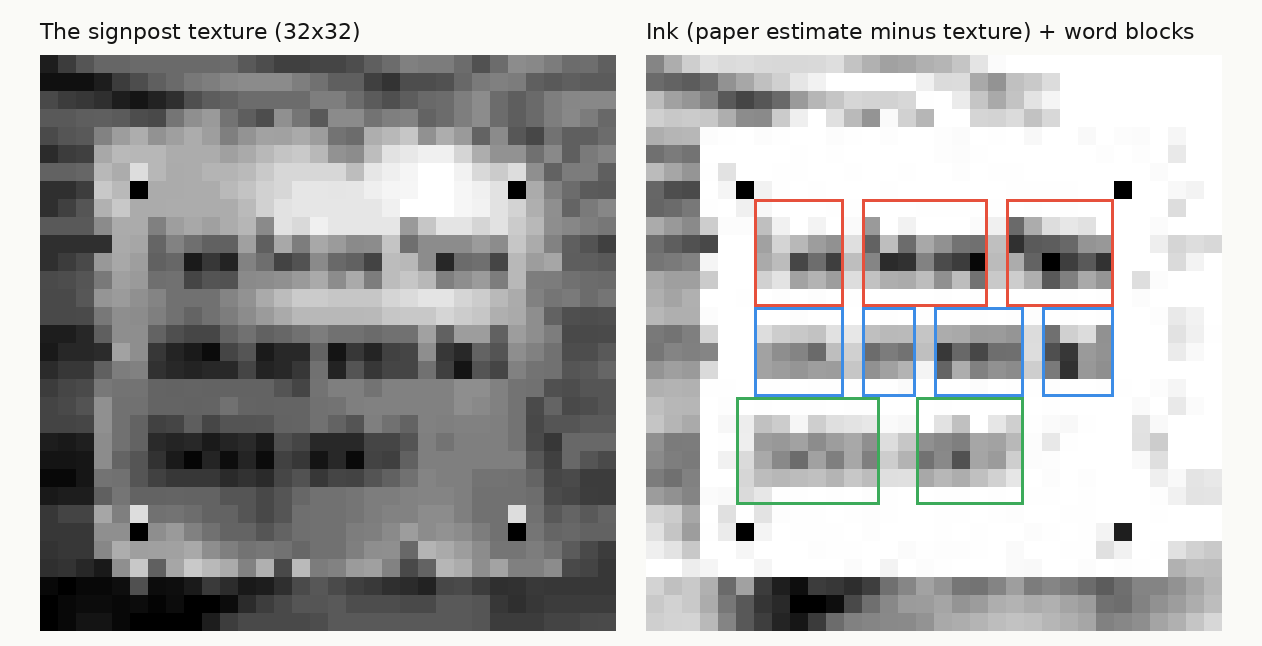
\includegraphics[width=0.85\linewidth]{sign_texture.png}
\caption{Left: the signpost texture, enlarged. Right: the \q{ink}, that is, how much darker each pixel is than the
painted board behind it (our estimate). The boxes are the word blocks we measured: three words on line~1, four on
line~2, two on line~3.}
\label{fig:texture}
\end{figure}

\paragraph{What the pixels show directly.}
\begin{itemize}
\item Three lines of text, at rows 9--12, 15--17 and 20--23 of the picture.
\item Clear gaps between words. Measured in pixels, the words are: line~1: 5, 7 and 6 pixels wide; line~2: 5, 3, 5 and
4; line~3: 8 and 6 (\cref{fig:texture}, right).
\item The board behind the text is not flat. It is painted with soft light and shadow, and this shading continues
under the letters.
\end{itemize}

\section{How we approach it}
\label{sec:method}
We use the same idea as our study of the courtyard plaque (\q{L is real 2401}, see the main report in this repository):
\emph{model, don't read}.
\begin{enumerate}
\item \textbf{Make a candidate.} Take a possible text, for example \q{I'm here. See / me as you go. / Hold on!}.
\item \textbf{Type it} in a real font of the 1990s, at a given size and spacing, on a larger canvas.
\item \textbf{Shrink it} to $32{\times}32$, the way paint programs did, and lay it on the painted board.
\item \textbf{Compare} the result with the real picture, pixel by pixel. The smaller the difference, the better the
candidate.
\end{enumerate}
\paragraph{The painted board.}
Because the board is shaded, we do not know exactly how bright it is behind each letter. We estimate it from the
surrounding board, which has no text, and we keep the uncertainty of that estimate. When we compare a candidate with
the picture, the board and the text are fitted \emph{together}: a candidate only scores well if some plausible board
plus its letters explains the pixels. (Technically, the board is a smooth random surface whose uncertainty is
integrated out; the score is a weighted least-squares error.)

\paragraph{Can this work at all?}
Before searching, we tested the method on fake signs made the same way, with known text. The answer is sobering.
\begin{itemize}
\item If we knew the board perfectly, the method would recover 28 of 30 lines exactly.
\item With the board only estimated, as for the real sign, it recovers between 0 and 4 of 30 lines exactly, and 10--33\,\% of
the words.
\end{itemize}
So the pixels alone cannot spell out every word. They can rule out a great deal, and they strongly favour some
shapes, but the final choice between close candidates has to use more than pixels: whether the sentence makes sense,
and how the developers wrote. This report keeps these two kinds of evidence apart.

\section{The first word: \q{I'm}}
\label{sec:im}
We started from one assumption: the first word is \q{I'm}. It has a capital stroke, an apostrophe and a short
\q{m}, which matches the first block well, and SM64's signs often talk in the first person (\q{I'm sleeping
because\ldots I'm sleepy}, \q{I'm serious.}, \q{I'll be back soon}). Testing it blind, without telling the search what
to expect, \q{I'm} came out 8th of 4{,}595 spellings that fit the block. So the assumption is consistent with the pixels.

\section{Sentences that make sense}
\label{sec:sentences}
Scoring word by word produces nonsense, so we scored whole signs. We wrote grammar patterns for what a three-line sign
can say, for example:
\begin{itemize}
\item \q{I'm here. \emph{Verb} / \emph{object} as/if/so \emph{subject verb} / \emph{closing}} (\q{See / me as you go! / Have fun!}),
\item \q{\ldots / \emph{object at the place}} (\q{Find / me at the top!}),
\item hand-written sign phrases in the style of SM64's own signs,
\end{itemize}
and filled them from word lists, keeping only words whose width fits the measured blocks. That gave about 3.2~billion
complete signs. A GPU scored all of them against the picture in under a minute: first each line alone, then the best
lines together with the shared board.

Simple width rules already settle several questions:
\begin{itemize}
\item The last word of line~2 is only 4~pixels wide: \q{go.}, \q{do!}, \q{sit} fit; \q{can!} (\q{find me if you
can!}) is far too wide.
\item \q{Hold} is too wide to end line~1, so a \q{Hold on} must be on line~3.
\item \q{Read} is too wide for the end of line~1.
\end{itemize}

\section{The font}
\label{sec:font}
With \q{I'm here} assumed, we fitted the font itself. We tried every font we have from the period: 2{,}897 fonts from
CorelDRAW, Bitstream, Adobe and Apple packages, IRIX workstations and more. For each font, its size, width, slant,
spacing, blur and stroke weight were fitted to the pixels of \q{I'm here}.
\begin{itemize}
\item \textbf{The writing is upright and set in a soft serif font.} The best fits are all of this type: Century~751
(an old-style Century), Benguiat, Bookman Light, ITC Cheltenham and Modern~880. A plain sans-serif like Helvetica fits
clearly worse.
\item \textbf{The exact font cannot be named}: the best few dozen fonts are within the noise of the fit.
\item \textbf{The process is clear}: about 4 texture pixels per letter height unit (roughly 24\,px type on a canvas six
times larger), letters 11--16\,\% narrower than normal, shrunk by plain pixel averaging, no extra brightening.
\item Two warnings for anyone repeating this: picture fonts and blobby display fonts can \q{win} with absurd settings
unless brightness and contrast are kept realistic, and a font collection made only of italics will make italics win by
slanting them back upright.
\end{itemize}
\begin{figure}[h]\centering
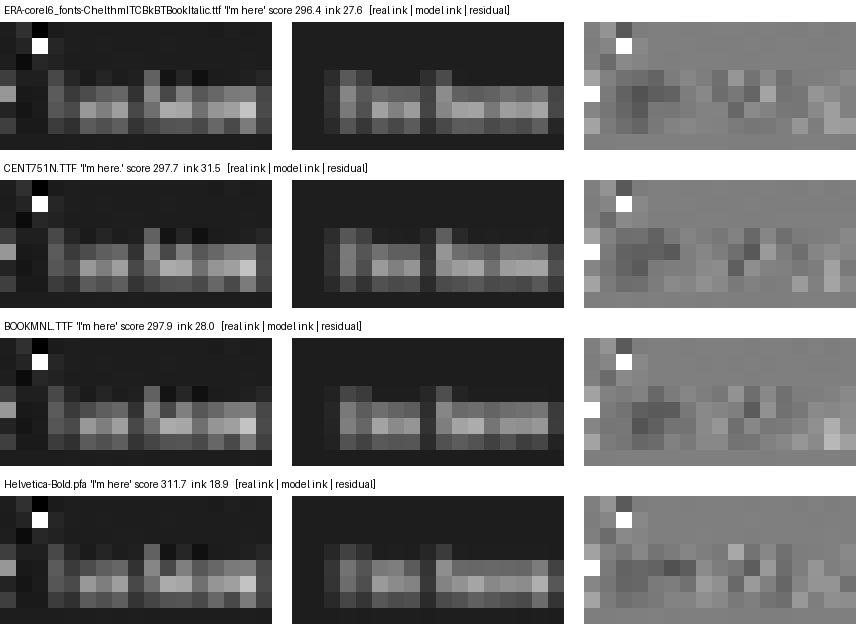
\includegraphics[width=0.95\linewidth]{fontfit_show.png}
\caption{\q{I'm here} fitted in three serif fonts and in Helvetica Bold. Each row: the real ink, the fitted ink, the
difference. At this size all good fonts look alike, which is why the exact font cannot be named.}
\label{fig:font}
\end{figure}

\section{Searching again with the right font}
\label{sec:search}
We then scored all 3.2~billion signs again, drawing every word in the four best serif fonts with their fitted settings
(\cref{fig:sentences}). This changed one thing clearly and left the rest as it was:
\begin{itemize}
\item \textbf{Line 1 is \q{I'm here. See}}, far ahead of every alternative (\q{Tell} was a close second with the earlier,
worse-fitting fonts; with the right font it falls 120 points behind).
\item \textbf{Line 2} is four short words. The pixels prefer \q{us} or \q{me} first, then a two-letter word (\q{as}),
then a short word in the third block, then a short ending. They like a two-letter third word (\q{we}) more than the
three-letter \q{you}.
\item \textbf{Line 3} is a closing phrase of two words. \q{Hold me!}, \q{Trust me!}, \q{Find me!} and \q{Turn left!}
are almost tied; \q{Hold on!} is close behind.
\end{itemize}

\begin{figure}[h]\centering
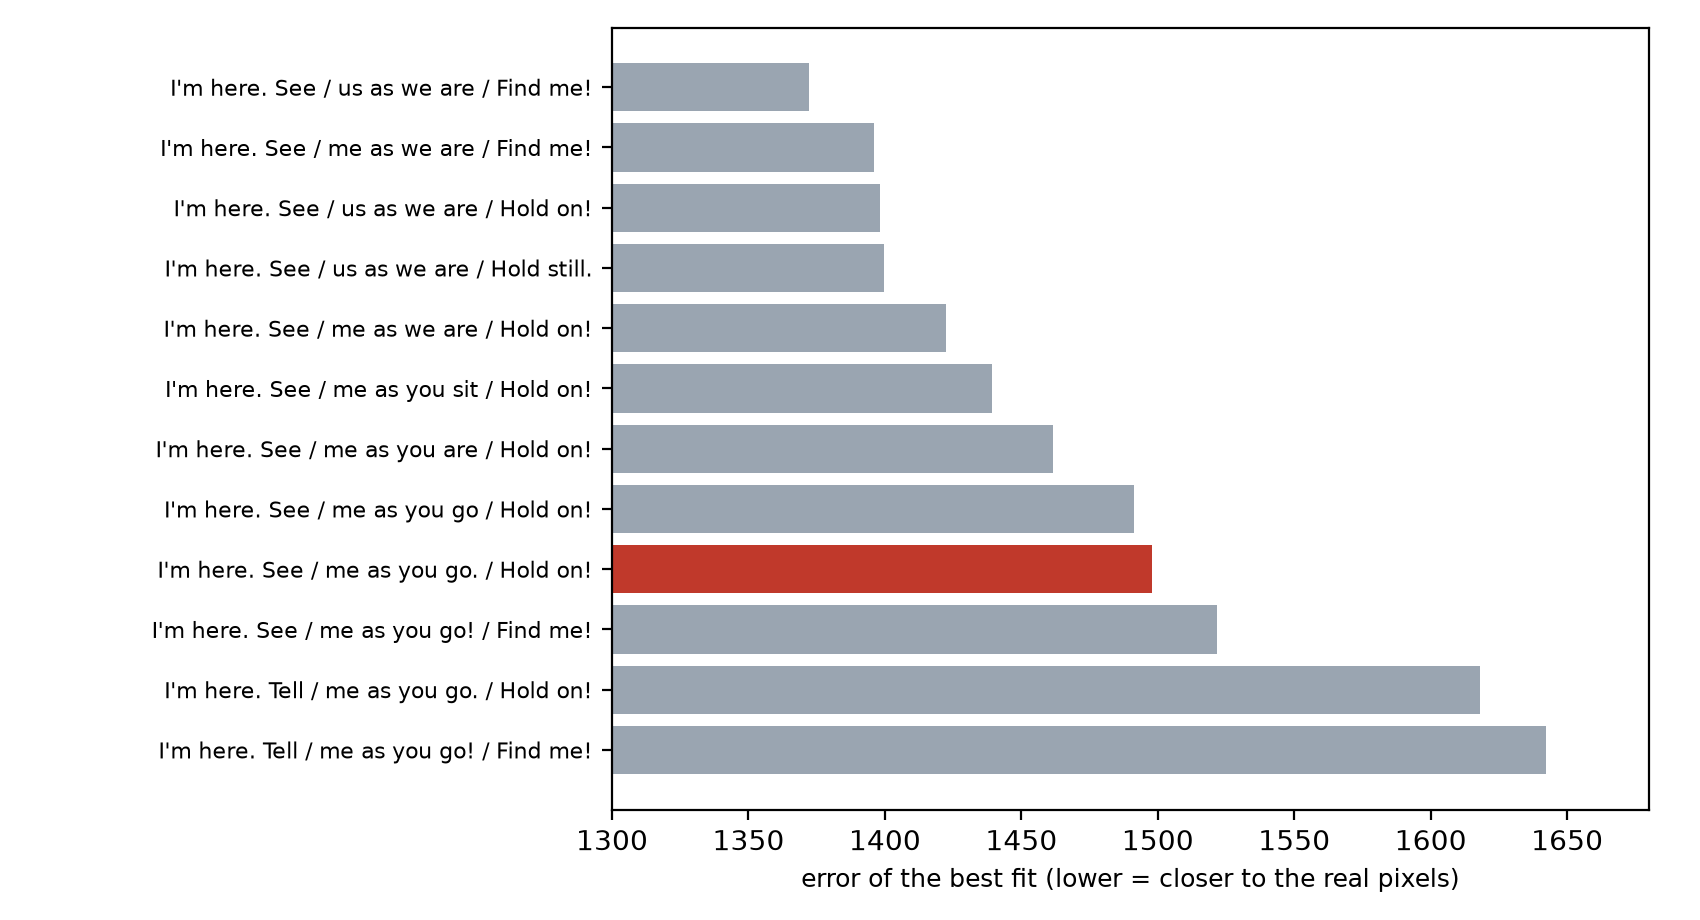
\includegraphics[width=0.85\linewidth]{sentences.png}
\caption{Sensible signs and how well they fit the pixels with the best font (lower is better). Red: our reading.
Differences of about 20 points are within the noise.}
\label{fig:sentences}
\end{figure}

\begin{table}[h]\centering\small
\begin{tabular}{lr}\toprule
sign & error (lower is better)\\\midrule
I'm here. See / us as we are / Find me! & 1372\\
I'm here. See / me as we are / Find me! & 1396\\
I'm here. See / us as we are / Hold on! & 1398\\
I'm here. See / me as we are / Hold on! & 1422\\
I'm here. See / me as you sit / Hold on! & 1439\\
I'm here. See / me as you are / Hold on! & 1462\\
\textbf{I'm here. See / me as you go. / Hold on!} & \textbf{1498}\\
I'm here. See / me as you go! / Find me! & 1522\\
I'm here. Tell / me as you go. / Hold on! & 1618\\
\bottomrule\end{tabular}
\caption{Selected sensible signs. The best possible string of any letters (not English) reaches about 1270.}
\label{tab:sentences}
\end{table}

\paragraph{What the pixels decide, and what they do not.}
By pixels alone, \q{I'm here. See / us as we are / Find me!} fits best among sensible sentences. Our reading is about 125
points behind it, mainly because of one word: the pixels prefer a two-letter word where we read \q{you}. Given the
calibration of \cref{sec:method} (with an estimated board, exact lines are recovered in at most 13\,\% of cases),
this is a preference, not a proof. The words that the pixels fix firmly are \q{I'm here. See}; the rest is chosen
among close candidates.

\section{Reading it as the developers wrote it}
\label{sec:japanese}
The English on SM64's textures was written by the Japanese team. On the courtyard plaque, \q{We hope so} is a direct
rendering of \jp{そう願っています}. So we asked of every candidate: what Japanese sentence would it come from, and would a
Japanese signpost say that?
\begin{table}[h]\centering\small
\begin{tabularx}{\linewidth}{p{4.0cm}p{4.3cm}X}\toprule
candidate & likely Japanese original & as a Japanese sign\\\midrule
\textbf{I'm here. See me as you go. Hold on!} & \jp{ここにいるよ。通りがかりに見ていってね。がんばってね！} & \textbf{very natural}:
\jp{見ていってね} (\q{have a look as you pass}) is standard shop and sign language; \jp{がんばって} is often rendered
\q{Hold on!}\\
I'm here. See us as we are. Find me! & \jp{ここにいるよ。ありのままの僕らを見て。見つけてね！} & poetic, like a song
lyric; odd for a signpost\\
I'm here. See me as we are. \ldots & \jp{ありのままの私を見て} with a slip in the pronoun & possible as a mistake\\
I'm here. See me as you sit. \ldots & \jp{座ってる間に見てね？} & nobody would say this\\
\bottomrule\end{tabularx}
\caption{Candidates read backwards into Japanese.}
\label{tab:japanese}
\end{table}

Our reading is the one that makes sense as a whole:
\begin{itemize}
\item \jp{ここにいるよ} -- \q{I'm here.} The sign introduces itself, just as SM64's signs speak in the first person.
\item \jp{通りがかりに見ていってね} -- \q{See me as you go.} Have a look at me as you pass by. Word-for-word school English
of the same kind as \q{We hope so}.
\item \jp{がんばってね！} -- \q{Hold on!} Hang in there, good luck: a natural thing for a sign to say to a player at the
start of an adventure.
\end{itemize}
The sign speaks as \q{I}, so it refers to itself as \q{me}, not \q{us}; the pixels allow this (\q{me} costs only about
24 points against \q{us}).

\section{Conclusion}
\label{sec:conclusion}
The wooden signpost in \emph{Super Mario 64} most likely reads
\begin{center}\Large\textit{I'm here. See me as you go. Hold on!}\end{center}
written in an upright soft serif font of the Century/Bookman kind, typed at about 24\,px and shrunk into the
$32{\times}32$ texture. How sure we are of each word:
\begin{center}\small\begin{tabular}{lp{9.5cm}l}\toprule
word & evidence & confidence\\\midrule
I'm & assumed; consistent with the pixels (8th of 4{,}595 blind) & assumed\\
here. & best in every search & high\\
See & best with the right font, 120 points ahead of \q{Tell} & high\\
me & the sign speaks as \q{I}; \q{us} fits 24 points better & moderate\\
as & a two-letter word in a 3-pixel block, top in the pixel ranking & moderate\\
you & pixels prefer a two-letter word here (\q{we}) & low\\
go. & fits the 4-pixel last block; \q{sit} and \q{are} fit better & low--moderate\\
Hold on! & among the best closings; \q{Hold me!} and \q{Find me!} fit slightly better & moderate\\
\bottomrule\end{tabular}\end{center}
The pixels settle the first line and the shape of the rest. The words of lines~2 and~3 are chosen as the sentence that
makes sense, both in English and as a translation from Japanese.

\paragraph{What we did not do.}
The analysis uses only the texture as it ships in the game. No leaked material was used, and no Nintendo data or
commercial fonts are distributed with this report.

\end{document}
